\documentclass[10pt]{article}

\usepackage[top=1in, bottom=1in, left=2cm, right=2cm]{geometry}
\usepackage{graphicx}

\def\eq1{y=\frac{x}{3x^2+x+1}}

\begin{document}

\title{Digital Tools For Finance}
\author{Sophia Kotsonis and Lionel Meise}
\date{\today}
\maketitle

\newpage

\tableofcontents


\newpage
\section{1. Part}
	\subsection{Math questions}

What is the value of x?
\begin{enumerate}
\item $x_1+5 = 6$\\
\item $x_2^2 = 4$\\
\item $x_3^{10} = 1$\\
\item $x_4^{3^5} = 1$\\

$...$\\
\item[10.] $x_{10} * 2 = 50$\\
\item[11.] $\log_{10}(x_{11}) = 100$\\
\item[12.] $\sqrt[3]{x_{12}} = 8$\\
\item[13.] $\frac{x_{13}}{6} = 2$\\
\item[14.] $x_{14}\left(\frac{3}{4}\right) = 16$\newline
\end{enumerate}

What is the value for these Greek letters?

$\pi + 3 = 5$\\
$\lambda / 4 = 10$\\

	\subsection{Writing style}

Other cool writing:
$$\left\{\left.\frac{x_a}{n}\right|_a a=2\right\}$$

Show the use of the displaystyle:\\
We have difficulties with reading this small fraction $\frac{x_a}{6}$\\
Now here $\displaystyle{\frac{x_a}{6}}$ we can clearly see the a under the x.
 
\newpage

\section{2. Part}
	\subsection{Table}
Here is a \textit{simple} but \textbf{good} looking table\\

\begin{tabular}{|c|c|c|c|}
\hline
$x$ & 1 & 2 & 3 \\ \hline
$f(x)$ & 10 & 11 & 12 \\
\hline
\end{tabular}\newline

	\subsection{Equation Array}
Here follows an example of an equation array
\begin{eqnarray}
5x^2&=&20\\
300x&=&60\\
x&\approx&\pm1.732
\end{eqnarray} \newline
 

	\subsection{Macros}
Here is my macro $\eq1$ \newline

	\subsection{Graphics}
\begin{center}	
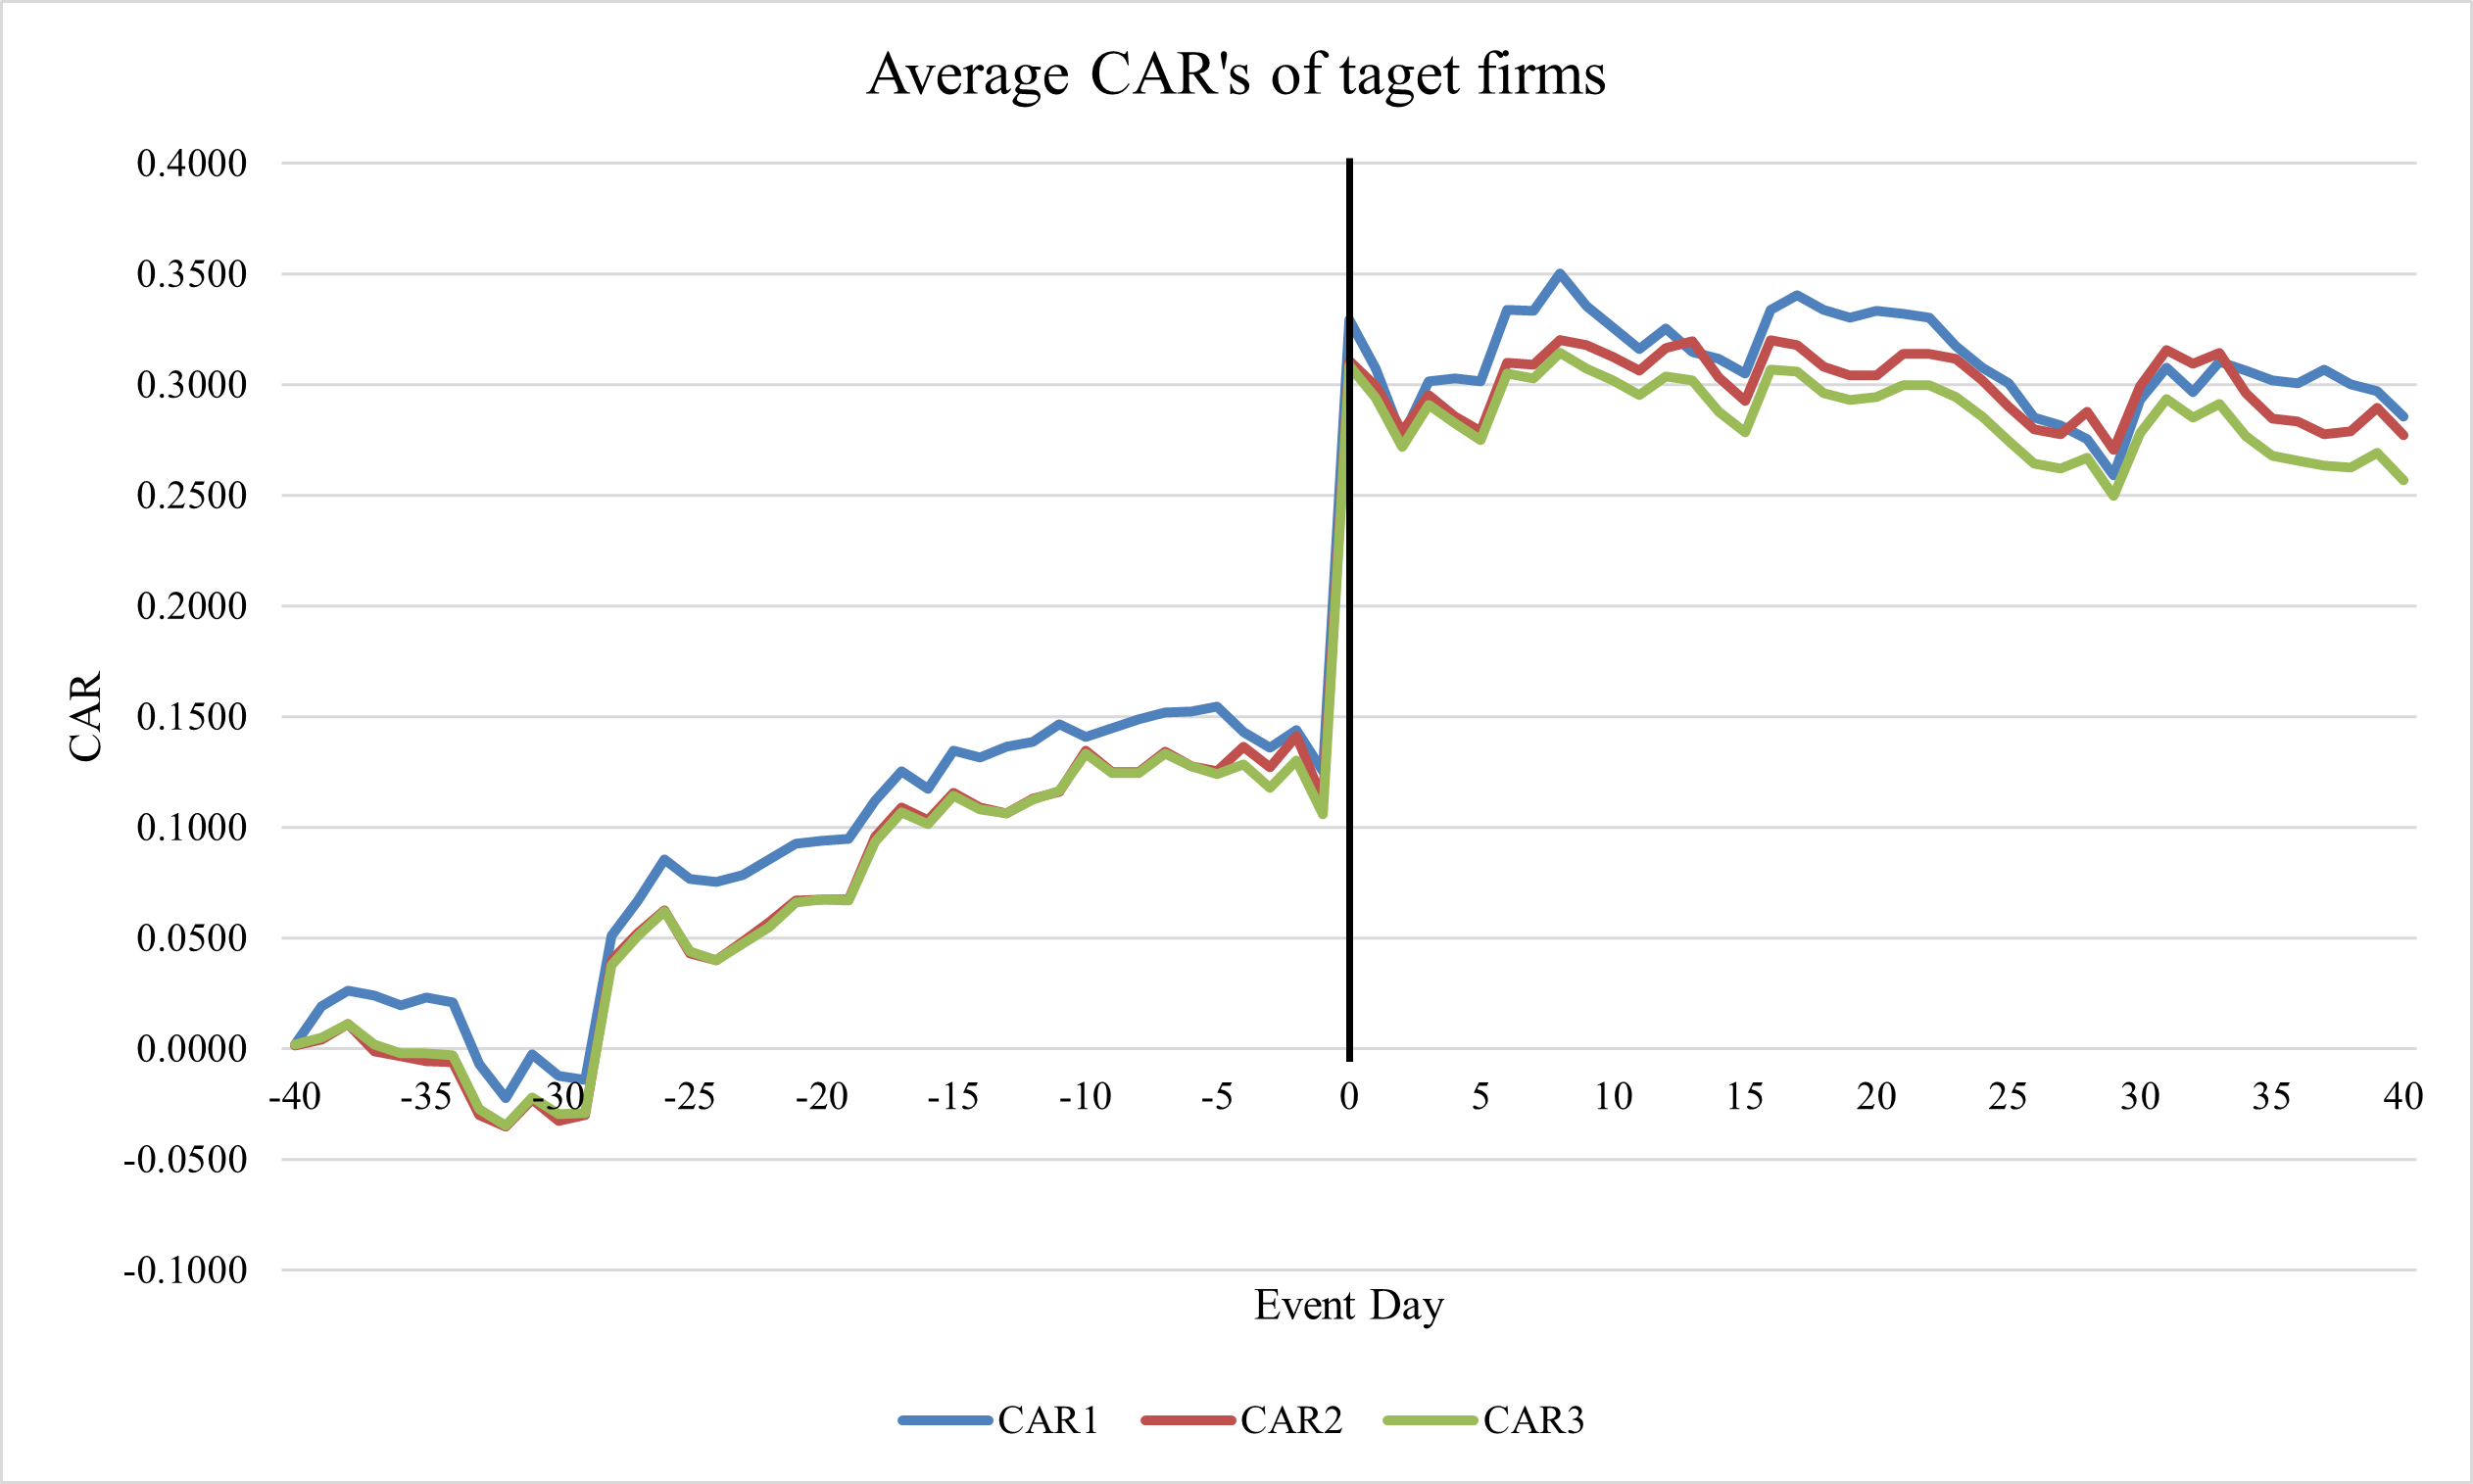
\includegraphics[scale=0.75]{Bild1.png}
\end{center}

\end{document}